
\subsubsection{Adaptivity Issues}
%%%%%%%%%%%%%%%%%%%%%%%%%%%%%%%%%%%%%%%%%%%%%%%%%%%%%%%%%%%%%%%%%%%%%
\royslide{Adaptivity and ParallelMesh}{
\begin{columns}
\begin{column}{.5\textwidth}
\begin{center}
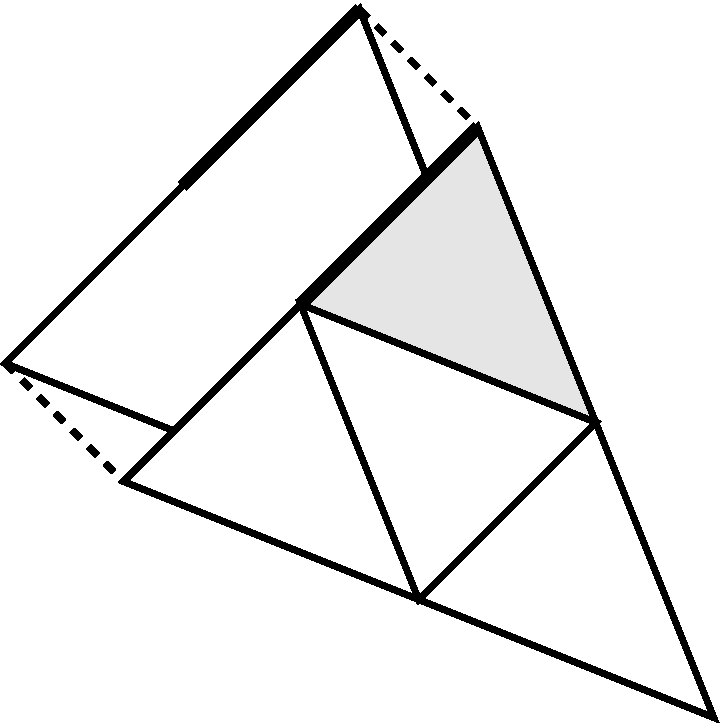
\includegraphics[width=.9\textwidth]{parallelism/adaptive}
\end{center}
\end{column}
\begin{column}{.5\textwidth}
\royitemizebegin{Challenges}
\item Reindexing elements, nodes, DoFs
\item Synchronization of ghost objects
\item Load balancing, Repartitioning
\royitemizeend
\end{column}
\end{columns}
}

%%%%%%%%%%%%%%%%%%%%%%%%%%%%%%%%%%%%%%%%%%%%%%%%%%%%%%%%%%%%%%%%%%%%%
\royslide{ParallelMesh Data Structure}{
\royitemizebegin{std::vector fails}
\item Not sparse
\item $O(N_E)$ storage cost
\royitemizeend
\royitemizebegin{std::map}
\item ``mapvector'' interface provides iterators
\item $O(log (N_E/N_P))$ lookup time without std::unsorted\_map
\item $O(1)$ lookup time with std::unsorted\_map
\royitemizeend
}



\subsubsection{Parallel Programming}
%%%%%%%%%%%%%%%%%%%%%%%%%%%%%%%%%%%%%%%%%%%%%%%%%%%%%%%%%%%%%%%%%%%%%
%\royslide{Parallel:: API}{
\begin{frame}[fragile]
\frametitle{Parallel:: API}
\royitemizebegin{Encapsulating MPI}
\item Improvement over MPI C++ interface
\item Makes code shorter, more legible
\royitemizeend

Example:
\small
\begin{lstlisting}
std::vector<Real> send, recv;
...
send_receive(dest_processor_id, send,
             source_processor_id, recv);
\end{lstlisting}
\end{frame}
%}



%%%%%%%%%%%%%%%%%%%%%%%%%%%%%%%%%%%%%%%%%%%%%%%%%%%%%%%%%%%%%%%%%%%%%
%\royslide{Parallel:: API}{
\begin{frame}[fragile,shrink]
\frametitle{Parallel:: API}

Instead of:
\begin{lstlisting}
if (dest_processor_id   == libMesh::processor_id() &&
    source_processor_id == libMesh::processor_id())
  recv = send;
#ifdef HAVE_MPI
else
  {
    unsigned int sendsize = send.size(), recvsize;
    MPI_Status status;
    MPI_Sendrecv(&sendsize, 1, datatype<unsigned int>(),
                 dest_processor_id, 0,
                 &recvsize, 1, datatype<unsigned int>(),
                 source_processor_id, 0,
                 libMesh::COMM_WORLD,
                 &status);

    recv.resize(recvsize);

    MPI_Sendrecv(sendsize ? &send[0] : NULL, sendsize, MPI_DOUBLE,
                 dest_processor_id, 0,
                 recvsize ? &recv[0] : NULL, recvsize, MPI_DOUBLE,
                 source_processor_id, 0,
                 libMesh::COMM_WORLD,
                 &status);
  }
#endif // HAVE_MPI
\end{lstlisting}
\end{frame}
%}

